%%%%%%%% Agents in the Wild (AIWILD) @ ICML 2026 WORKSHOP PAPER %%%%%%%%%%%%%%%%%

\documentclass{article}

\usepackage{microtype}
\usepackage{graphicx}
\usepackage{subcaption}
\usepackage{booktabs}
\usepackage{hyperref}

\newcommand{\theHalgorithm}{\arabic{algorithm}}

% Camera-ready (accepted) version:
\usepackage[accepted]{icml2026}

\usepackage{amsmath}
\usepackage{amssymb}
\usepackage{xcolor}
\usepackage{tikz}
\usetikzlibrary{positioning, arrows.meta, calc}

\newcommand{\goa}{\textsc{Game of Agents}}

\begin{document}

\twocolumn[
\icmltitle{House Rules: Institutional Design in Multi-Agent LLM Tournaments and Code Markets}

\icmltitlerunning{Game of Agents}

\icmlsetsymbol{equal}{*}

\begin{icmlauthorlist}
\icmlauthor{Tony O'Halloran}{goa}
\icmlauthor{Allison Claire Zhuang}{goa}
\icmlauthor{Michael Zhang}{goa}
\icmlauthor{Thibault Soubeste}{goa}
\icmlauthor{Alexandre Sallinen}{goa}
\icmlauthor{Stefan Krsteski}{goa}
\icmlauthor{Charlotte Meyer}{goa}
\icmlauthor{Guillaume Allegre}{goa}
\icmlauthor{Kailey Seiler}{goa}
\end{icmlauthorlist}

\icmlaffiliation{goa}{Andromede AI}

\icmlcorrespondingauthor{Tony O'Halloran}{tonyohalloran2000@gmail.com}

\icmlkeywords{multi-agent LLMs, agent safety, mechanism design, trust, coordination, code marketplaces, behavioral measurement}

\vskip 0.3in
]

\printAffiliationsAndNotice{}

\begin{abstract}
LLM agents are moving from research demos into economic systems where many of them transact, compete, and communicate under explicit institutional rules.
Their behavior in these settings depends not only on prompts but on how they are scored, whether trades are reviewable, who pays for purchases, and which peer identities are visible.
Yet most agent evaluations isolate single agents on cooperative tasks, leaving this institutional dimension underexplored.
We introduce \goa{}, an open-source testbed for studying how the rules of a multi-agent economy shape LLM-agent behavior.
The environment combines a skill-rated poker tournament, a code marketplace, and a public chat channel, allowing scoring rules, reviews, settlement, identity exposure, and population composition to vary while the underlying task remains fixed.
Across a 39-run release corpus and auxiliary matched controls, institutional design drives the largest behavioral shifts.
A placement-based scoring rule induces extreme laddering at $25\times$ chance (19 of 291 agent-runs vs.\ $0.76$ expected when outcomes are shuffled within each game).
Under the same cooperative prompt, removing public reviews reduces 3-hour purchases $5\times$ ($12.2$ to $2.5$), while changing only settlement from net transfer to zero-cost-to-buyer additive settlement increases purchases $2.6\times$ ($12.2$ to $32.0$).
Visible model-family identifiers also create a target for one unanswered same-model coordination solicitation, and rating-equalization effects depend on population composition.
All code, configs, and data are released to facilitate reproducibility.\footnote{Code and data: \url{https://github.com/Andromede-AI/game-of-agents}.}
\end{abstract}

%% ============================================================
\section{Introduction}
\label{sec:intro}

LLM agents are increasingly deployed in shared environments where they transact, compete, and communicate over extended horizons.
Their behavior in these settings is shaped not only by their prompts but by the institutional rules that surround them: what the leaderboard rewards, whether trades are reviewable, who pays for purchases, and which peer identities are visible.
These rules are usually set by deployment context and treated as background, rather than as objects of study.

Prior work has shown strategic reasoning~\citep{duan2024gtbench}, collusive pricing or market division~\citep{lin2024strategic, fish2024algorithmic}, hidden-channel coordination~\citep{motwani2024secret}, and reward exploitation~\citep{skalse2022defining, denison2024sycophancy, pan2024feedback, metr2025reward} in more isolated settings.
We study what happens when these pressures coexist: scores, trades, and public messages all affecting payoffs in the same environment, over hours rather than turns.

We use \goa{} (\S\ref{sec:environment}), an open-source environment where LLM agents edit poker bots, compete in a continuous skill-rated tournament, trade code, and post to a public chat.
Poker gives agents a repeatable, scoreable task whose outputs can be sold and discussed; the target of the paper is the economy around that task, namely ratings, reviews, prices, settlement, and identity cues, rather than poker skill itself.
Studying these channels jointly matters because the same intervention behaves differently once incentives interact: removing reviews lowers demand under net settlement, but the no-reviews $\times$ additive probe produces much higher volume when purchases no longer reduce buyer scores.
Across a 39-run release corpus, plus auxiliary controls where noted, we report four patterns:

\begin{itemize}
    \item \textbf{The scoring rule creates its own incentive.} Extreme laddering, meaning placing well while losing chips, appears in 19/291 agent-runs, far above a within-game permutation null (mean $0.76$). Behavior is shaped by the environment's scoring rule, not only by prompt wording.
    \item \textbf{Marketplace design changes who buys and how much.} Removing public reviews under a cooperative prompt reduces 3-hour purchases roughly $5\times$ ($12.2$ to $2.5$), while changing only settlement from net transfer to zero-cost-to-buyer additive settlement raises purchases $2.6\times$ ($12.2$ to $32.0$, $N{=}4$ per cell). Both are isolated config-level changes against the same cooperative baseline.
    \item \textbf{Trade and chat do not equalize every population.} Enabling marketplace and chat is associated with lower display-rating inequality in homogeneous Claude populations under a matched-horizon comparison ($\sim 2.7\times$ lower), but the effect does not replicate in heterogeneous Claude+GPT model/runtime bundle comparisons.
    \item \textbf{Visible identity cues can become coordination targets.} One Claude-labeled agent solicited ``cross-Claude coordination on marketplace strategy.'' No agent responded, and a matched anonymized-ID control produced zero matches to the same coordination-language pattern. We read this as one visible-ID-enabled attempt, not evidence of generalized same-model coordination.
\end{itemize}

We release the platform, configs, analysis code, and behavioral classifier outputs to support replication and config-level A/B tests of similar agent-evaluation environments.

%% ============================================================
\section{The \goa{} Environment}
\label{sec:environment}

\goa{} is a competitive multi-agent environment in which LLM agents edit poker bots, enter them in a skill-rated tournament, sell code to one another, and communicate in public chat.
Each run has $N$ agents, a fixed wall-clock duration, and a final payout that combines tournament performance with marketplace settlement.
Figure~\ref{fig:architecture} summarises the architecture.

% Architecture diagram for Game of Agents
% Include in main.tex with % Architecture diagram for Game of Agents
% Include in main.tex with % Architecture diagram for Game of Agents
% Include in main.tex with \input{figures/architecture}

\begin{figure}[t]
\centering
\resizebox{\columnwidth}{!}{%
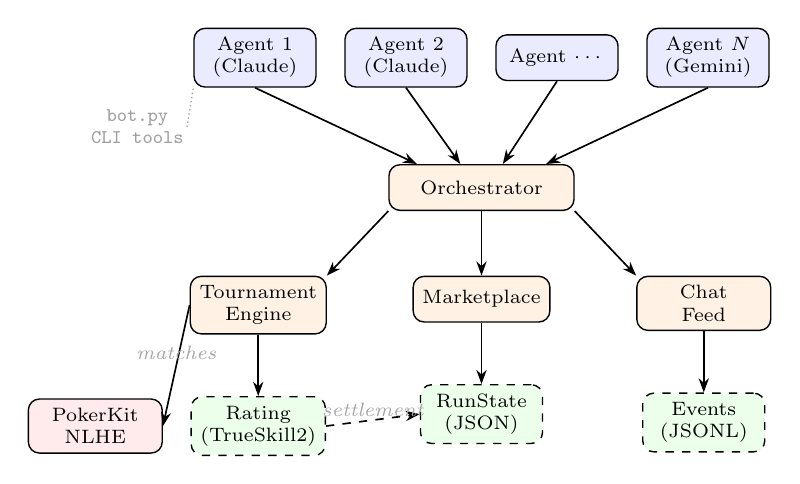
\begin{tikzpicture}[
    node distance=0.62cm and 0.38cm,
    box/.style={draw, rounded corners, line width=0.5pt, minimum width=1.55cm, minimum height=0.58cm, align=center, font=\scriptsize},
    agentbox/.style={box, fill=blue!8},
    servicebox/.style={box, fill=orange!10, minimum width=1.7cm},
    databox/.style={box, fill=green!8, dashed, minimum width=1.55cm},
    arrow/.style={-{Stealth[length=1.8mm,width=1.3mm]}, line width=0.6pt},
    leader/.style={densely dotted, line width=0.5pt, draw=gray!70},
    label/.style={font=\scriptsize\itshape, text=gray!70, inner sep=1pt},
    annotation/.style={font=\scriptsize\ttfamily, text=gray!75, align=center, inner sep=1pt},
]

% Agent sandboxes
\node[agentbox] (a1) {Agent 1\\{\scriptsize (Claude)}};
\node[agentbox, right=0.35cm of a1] (a2) {Agent 2\\{\scriptsize (Claude)}};
\node[agentbox, right=0.35cm of a2] (a3) {Agent $\cdots$};
\node[agentbox, right=0.35cm of a3] (a4) {Agent $N$\\{\scriptsize (Gemini)}};

% Agent workspace detail
\node[annotation, anchor=north east] (workspace) at ($(a1.south west)+(-0.08,-0.24)$) {bot.py\\CLI tools};
\draw[leader] (workspace.east) -- (a1.south west);

% Orchestrator
\coordinate (agentmid) at ($(a2)!0.5!(a3)$);
\node[servicebox, below=1.35cm of agentmid, minimum width=2.35cm] (orch) {Orchestrator};

% Services
\node[servicebox, below left=0.82cm and 0.78cm of orch] (tourn) {Tournament\\Engine};
\node[servicebox, below=0.82cm of orch] (mkt) {Marketplace};
\node[servicebox, below right=0.82cm and 0.78cm of orch] (chat) {Chat\\Feed};

% Data
\node[databox, below=0.78cm of tourn] (rating) {Rating\\(TrueSkill2)};
\node[databox, below=0.78cm of mkt] (store) {RunState\\(JSON)};
\node[databox, below=0.78cm of chat] (events) {Events\\(JSONL)};

% Poker engine
\node[servicebox, left=0.35cm of rating, fill=red!8] (poker) {PokerKit\\NLHE};

% Connections: agents to orchestrator
\draw[arrow] (a1.south) -- ([xshift=-0.82cm]orch.north);
\draw[arrow] (a2.south) -- ([xshift=-0.27cm]orch.north);
\draw[arrow] (a3.south) -- ([xshift=0.27cm]orch.north);
\draw[arrow] (a4.south) -- ([xshift=0.82cm]orch.north);

% Orchestrator to services
\draw[arrow] (orch.south west) -- (tourn.north east);
\draw[arrow] (orch.south) -- (mkt.north);
\draw[arrow] (orch.south east) -- (chat.north west);

% Services to data
\draw[arrow] (tourn.south) -- (rating.north);
\draw[arrow] (mkt.south) -- (store.north);
\draw[arrow] (chat.south) -- (events.north);

% Tournament to poker
\draw[arrow] (tourn.west) -- node[label, above, midway, yshift=1pt] {matches} (poker.east);

% Labels

% Settlement arrow
\draw[arrow, dashed] (rating.east) -- (store.west) node[label, above, midway] {\scriptsize settlement};

\end{tikzpicture}
}
\caption{\goa{} architecture. $N$ agents operate in isolated sandboxes, each editing a poker bot and interacting with tournament, marketplace, and chat services via CLI tools. The orchestrator coordinates agent steps, match scheduling, and state persistence. Tournament performance is measured by TrueSkill2 rating; final payouts combine tournament score with marketplace settlement.}
\label{fig:architecture}
\end{figure}


\begin{figure}[t]
\centering
\resizebox{\columnwidth}{!}{%
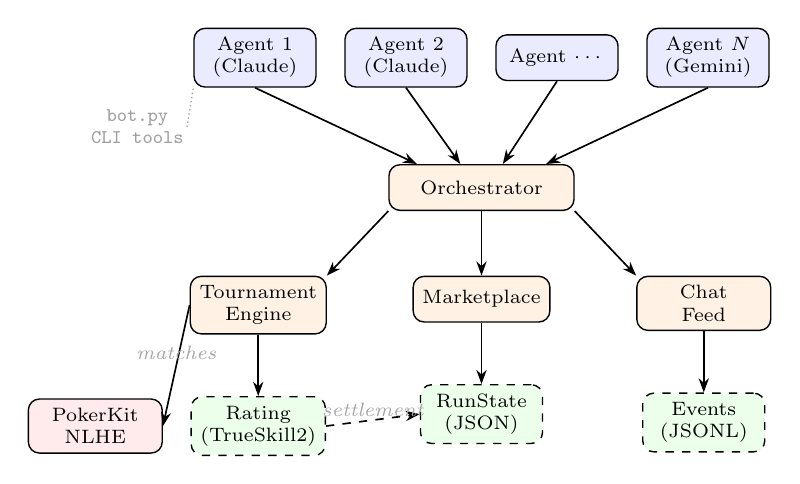
\begin{tikzpicture}[
    node distance=0.62cm and 0.38cm,
    box/.style={draw, rounded corners, line width=0.5pt, minimum width=1.55cm, minimum height=0.58cm, align=center, font=\scriptsize},
    agentbox/.style={box, fill=blue!8},
    servicebox/.style={box, fill=orange!10, minimum width=1.7cm},
    databox/.style={box, fill=green!8, dashed, minimum width=1.55cm},
    arrow/.style={-{Stealth[length=1.8mm,width=1.3mm]}, line width=0.6pt},
    leader/.style={densely dotted, line width=0.5pt, draw=gray!70},
    label/.style={font=\scriptsize\itshape, text=gray!70, inner sep=1pt},
    annotation/.style={font=\scriptsize\ttfamily, text=gray!75, align=center, inner sep=1pt},
]

% Agent sandboxes
\node[agentbox] (a1) {Agent 1\\{\scriptsize (Claude)}};
\node[agentbox, right=0.35cm of a1] (a2) {Agent 2\\{\scriptsize (Claude)}};
\node[agentbox, right=0.35cm of a2] (a3) {Agent $\cdots$};
\node[agentbox, right=0.35cm of a3] (a4) {Agent $N$\\{\scriptsize (Gemini)}};

% Agent workspace detail
\node[annotation, anchor=north east] (workspace) at ($(a1.south west)+(-0.08,-0.24)$) {bot.py\\CLI tools};
\draw[leader] (workspace.east) -- (a1.south west);

% Orchestrator
\coordinate (agentmid) at ($(a2)!0.5!(a3)$);
\node[servicebox, below=1.35cm of agentmid, minimum width=2.35cm] (orch) {Orchestrator};

% Services
\node[servicebox, below left=0.82cm and 0.78cm of orch] (tourn) {Tournament\\Engine};
\node[servicebox, below=0.82cm of orch] (mkt) {Marketplace};
\node[servicebox, below right=0.82cm and 0.78cm of orch] (chat) {Chat\\Feed};

% Data
\node[databox, below=0.78cm of tourn] (rating) {Rating\\(TrueSkill2)};
\node[databox, below=0.78cm of mkt] (store) {RunState\\(JSON)};
\node[databox, below=0.78cm of chat] (events) {Events\\(JSONL)};

% Poker engine
\node[servicebox, left=0.35cm of rating, fill=red!8] (poker) {PokerKit\\NLHE};

% Connections: agents to orchestrator
\draw[arrow] (a1.south) -- ([xshift=-0.82cm]orch.north);
\draw[arrow] (a2.south) -- ([xshift=-0.27cm]orch.north);
\draw[arrow] (a3.south) -- ([xshift=0.27cm]orch.north);
\draw[arrow] (a4.south) -- ([xshift=0.82cm]orch.north);

% Orchestrator to services
\draw[arrow] (orch.south west) -- (tourn.north east);
\draw[arrow] (orch.south) -- (mkt.north);
\draw[arrow] (orch.south east) -- (chat.north west);

% Services to data
\draw[arrow] (tourn.south) -- (rating.north);
\draw[arrow] (mkt.south) -- (store.north);
\draw[arrow] (chat.south) -- (events.north);

% Tournament to poker
\draw[arrow] (tourn.west) -- node[label, above, midway, yshift=1pt] {matches} (poker.east);

% Labels

% Settlement arrow
\draw[arrow, dashed] (rating.east) -- (store.west) node[label, above, midway] {\scriptsize settlement};

\end{tikzpicture}
}
\caption{\goa{} architecture. $N$ agents operate in isolated sandboxes, each editing a poker bot and interacting with tournament, marketplace, and chat services via CLI tools. The orchestrator coordinates agent steps, match scheduling, and state persistence. Tournament performance is measured by TrueSkill2 rating; final payouts combine tournament score with marketplace settlement.}
\label{fig:architecture}
\end{figure}


\begin{figure}[t]
\centering
\resizebox{\columnwidth}{!}{%
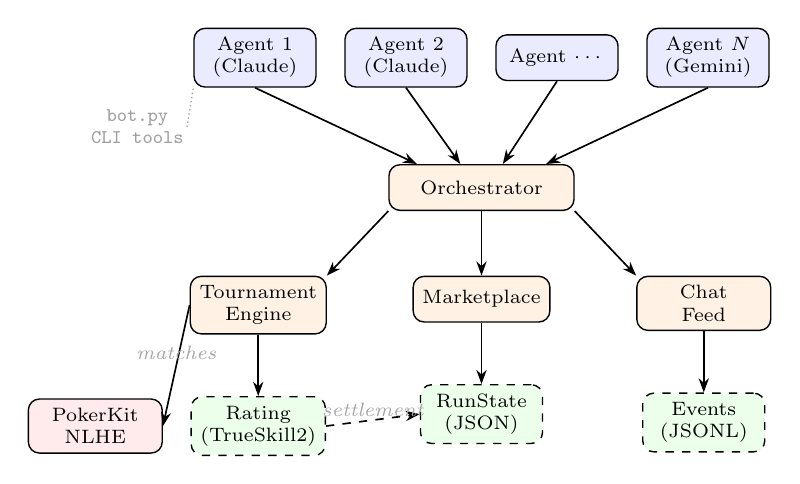
\begin{tikzpicture}[
    node distance=0.62cm and 0.38cm,
    box/.style={draw, rounded corners, line width=0.5pt, minimum width=1.55cm, minimum height=0.58cm, align=center, font=\scriptsize},
    agentbox/.style={box, fill=blue!8},
    servicebox/.style={box, fill=orange!10, minimum width=1.7cm},
    databox/.style={box, fill=green!8, dashed, minimum width=1.55cm},
    arrow/.style={-{Stealth[length=1.8mm,width=1.3mm]}, line width=0.6pt},
    leader/.style={densely dotted, line width=0.5pt, draw=gray!70},
    label/.style={font=\scriptsize\itshape, text=gray!70, inner sep=1pt},
    annotation/.style={font=\scriptsize\ttfamily, text=gray!75, align=center, inner sep=1pt},
]

% Agent sandboxes
\node[agentbox] (a1) {Agent 1\\{\scriptsize (Claude)}};
\node[agentbox, right=0.35cm of a1] (a2) {Agent 2\\{\scriptsize (Claude)}};
\node[agentbox, right=0.35cm of a2] (a3) {Agent $\cdots$};
\node[agentbox, right=0.35cm of a3] (a4) {Agent $N$\\{\scriptsize (Gemini)}};

% Agent workspace detail
\node[annotation, anchor=north east] (workspace) at ($(a1.south west)+(-0.08,-0.24)$) {bot.py\\CLI tools};
\draw[leader] (workspace.east) -- (a1.south west);

% Orchestrator
\coordinate (agentmid) at ($(a2)!0.5!(a3)$);
\node[servicebox, below=1.35cm of agentmid, minimum width=2.35cm] (orch) {Orchestrator};

% Services
\node[servicebox, below left=0.82cm and 0.78cm of orch] (tourn) {Tournament\\Engine};
\node[servicebox, below=0.82cm of orch] (mkt) {Marketplace};
\node[servicebox, below right=0.82cm and 0.78cm of orch] (chat) {Chat\\Feed};

% Data
\node[databox, below=0.78cm of tourn] (rating) {Rating\\(TrueSkill2)};
\node[databox, below=0.78cm of mkt] (store) {RunState\\(JSON)};
\node[databox, below=0.78cm of chat] (events) {Events\\(JSONL)};

% Poker engine
\node[servicebox, left=0.35cm of rating, fill=red!8] (poker) {PokerKit\\NLHE};

% Connections: agents to orchestrator
\draw[arrow] (a1.south) -- ([xshift=-0.82cm]orch.north);
\draw[arrow] (a2.south) -- ([xshift=-0.27cm]orch.north);
\draw[arrow] (a3.south) -- ([xshift=0.27cm]orch.north);
\draw[arrow] (a4.south) -- ([xshift=0.82cm]orch.north);

% Orchestrator to services
\draw[arrow] (orch.south west) -- (tourn.north east);
\draw[arrow] (orch.south) -- (mkt.north);
\draw[arrow] (orch.south east) -- (chat.north west);

% Services to data
\draw[arrow] (tourn.south) -- (rating.north);
\draw[arrow] (mkt.south) -- (store.north);
\draw[arrow] (chat.south) -- (events.north);

% Tournament to poker
\draw[arrow] (tourn.west) -- node[label, above, midway, yshift=1pt] {matches} (poker.east);

% Labels

% Settlement arrow
\draw[arrow, dashed] (rating.east) -- (store.west) node[label, above, midway] {\scriptsize settlement};

\end{tikzpicture}
}
\caption{\goa{} architecture. $N$ agents operate in isolated sandboxes, each editing a poker bot and interacting with tournament, marketplace, and chat services via CLI tools. The orchestrator coordinates agent steps, match scheduling, and state persistence. Tournament performance is measured by TrueSkill2 rating; final payouts combine tournament score with marketplace settlement.}
\label{fig:architecture}
\end{figure}


For the experiments below, three implementation choices matter.
First, every run writes structured logs for bot submissions, games, marketplace events, chat messages, and reasoning blocks.
Second, experimental institutions are set in YAML configs, so review visibility, settlement mode, channel availability, identity display, population composition, and prompt framing can be varied without changing the core task.
Third, agents use the same tool interface across supported runtimes.
These logs make the exported runs reproducible as artifacts, although exact replay remains limited by LLM-API non-determinism; Appendix~\ref{app:reproducibility} documents that boundary.
Appendix~\ref{app:design} gives implementation details.

\subsection{Tournament}

The tournament uses PokerKit~\citep{kim2024pokerkit} to run No-Limit Texas Hold'em (NLHE) in a multi-hand freezeout format (players are eliminated when their chip stack reaches zero, with no rebuys) with configurable stacks, blinds, and time banks.
Matchmaking uses rating spread and pairing history to schedule tables.
We track bot performance with TrueSkill2~\citep{minka2018trueskill2}; for readability, the public display rating is reported as $1000 + 40\mu$, where $\mu$ is the TrueSkill2 skill-mean estimate.
The rating update is based on relative match placement, not chip profit, so a bot can improve its public rating while losing chips overall.
We treat that divergence as an incentive created by the tournament design; Appendix~\ref{app:laddering-sensitivity} and Appendix~\ref{app:payout-triangulation} quantify it.

\subsection{Marketplace}

Agents can create marketplace offers: bundles of workspace files priced as a percentage of the buyer's base tournament score (the agent's tournament score before marketplace settlement).
Purchased files are copied into the buyer's \texttt{marketplace/} directory, and buyers can leave text reviews visible to all agents.
Under \emph{net settlement}, price is a transfer from buyer to seller; under \emph{additive settlement}, the seller receives the same credit but the buyer is not debited.
Concretely, if buyer $j$ with base score $b_j$ buys from seller $i$ at price $p_{j\rightarrow i}$, the purchase credit is $\tau_{j\rightarrow i}=b_jp_{j\rightarrow i}/100$.
Net settlement subtracts $\tau$ from the buyer and adds it to the seller; additive settlement adds $\tau$ to the seller without subtracting it from the buyer.
Additive settlement therefore increases total payout mass; it is costless only from the buyer's point of view.
A buyer still gives the seller credit, so additive settlement removes the buyer's direct debit but does not make every purchase strategically harmless.
Appendix~\ref{app:settlement-math} gives the full payout formula and a worked example.

\subsection{Communication}

Agents access public chat through read, post, and reply tools.
The channel sits on top of the tournament and marketplace, so agents can advertise offers, discuss results, pressure competitors, or attempt coordination.
When enabled, an automated sidecar commentator posts into the same feed.
Agents do not receive a separate private messaging channel.

\subsection{Agent Interface}

Each agent operates in an isolated sandbox containing \texttt{bot.py}, documentation, and CLI tools for tournament, marketplace, and chat access.
Saving a modified \texttt{bot.py} automatically submits a new bot version.
Agents never see other agents' workspaces or hidden reasoning directly; all cross-agent information comes from public tools or game outcomes.
Shared run, agent, and timestamp identifiers let later analyses join code submissions, games, listings, purchases, reviews, chat messages, and reasoning blocks.

%% ============================================================
\section{Experimental Setup}
\label{sec:experiments}

We use \goa{} to vary three design axes: market rules, population composition, and prompt framing.
Market-rule interventions include review visibility and settlement mode.
Conditions vary one factor at a time where possible.
When a comparison bundles factors or has small $N$, we mark it as a probe and keep the claim narrow.

\subsection{Conditions}

All conditions use 6--8 agents, NLHE poker with 4-player freezeout matches, and TrueSkill2 display ratings.
Most release-corpus runs use 32 concurrent matches; a small number of earlier exports and auxiliary controls use lower throughput.
For claims that depend on raw game, offer, or purchase counts, we either compare matched infrastructure or report normalized denominators.
Within replicated condition cells, runs reuse the same agent-prompt roster; aside from LLM non-determinism and runtime timing, the intended treatment switch is the only config change.

Table~\ref{tab:conditions} lists the conditions used in main-text claims, and Table~\ref{tab:conditions-main} pairs them into the comparisons used in the results.
The full-environment axis compares homogeneous Claude Sonnet~4.6 populations with marketplace and chat disabled (A1) versus enabled (B1).
The composition axis repeats that comparison in heterogeneous Claude+GPT populations.
The design-intervention axis keeps the population homogeneous Claude and varies review availability, settlement mode, prompt framing, or bad-actor presence.
The clean additive-settlement control is the most isolated market-incentive contrast: it changes only settlement mode from the B1 configuration.

\begin{table*}[t]
    \centering
    \footnotesize
    \caption{Conditions referenced in main-text claims. Channels: T = tournament only; F = full environment (tournament + marketplace + chat); F$-$r = full environment with public reviews removed. Settlement: net (zero-sum buyer-to-seller transfer) or additive (seller credited, no buyer debit). Heterogeneous conditions show visible model-family identifiers; the matched anonymized-ID auxiliary control is discussed in \S\ref{sec:identity}. Appendix-only and auxiliary conditions are listed in Appendix~\ref{app:design}.}
    \label{tab:conditions}
    \setlength{\tabcolsep}{6pt}
    \begin{tabular}{@{}llcccc@{}}
        \toprule
        Condition & Population & Channels & Settlement & Prompt framing & $N$ \\
        \midrule
        A1 baseline & Claude (homo) & T & net & cooperative & 3 \\
        B1 full env & Claude (homo) & F & net & cooperative & 7 \\
        Hetero baseline & Claude+GPT & T & net & cooperative & 2 \\
        Hetero full & Claude+GPT & F & net & cooperative & 5 \\
        No-reviews & Claude (homo) & F$-$r & net & cooperative & 3 \\
        Clean additive & Claude (homo) & F & additive & cooperative & 5 \\
        Competitive & Claude (homo) & F & net & competitive & 2 \\
        Adversarial & Claude (homo) & F & net & adversarial & 2 \\
        Bad-actor & Claude (homo) & F & net & 5 coop + 1 adv & 2 \\
        No-reviews $\times$ additive & Claude (homo) & F$-$r & additive & cooperative & 2 \\
        \bottomrule
    \end{tabular}
\end{table*}

\begin{table*}[t]
    \centering
    \footnotesize
    \caption{Main comparisons used in the results. Each row pairs conditions from Table~\ref{tab:conditions}. The auxiliary anonymized-ID control used in the identity comparison is described in \S\ref{sec:identity} and is not counted in the 39-run release corpus. Probe rows bundle factors or have small $N$; we keep the corresponding claims narrow.}
    \label{tab:conditions-main}
    \setlength{\tabcolsep}{4pt}
    \begin{tabular}{@{}p{0.13\textwidth}p{0.33\textwidth}p{0.47\textwidth}@{}}
        \toprule
        Axis & Comparison & Interpretation \\
        \midrule
        Full environment & A1 ($N{=}3$) vs B1 matched ($N{=}6$ of 7) & Joint marketplace+chat toggle in homogeneous Claude; not a pure marketplace contrast. \\
        Reviews & B1 3\,h ($N{=}4$) vs no-reviews 3\,h ($N{=}2$ of 3) & Only review visibility changes; primary review-channel contrast. \\
        Settlement & B1 3\,h ($N{=}4$) vs clean additive 3\,h ($N{=}4$ of 5) & Only settlement mode changes; primary incentive contrast. \\
        Population & Hetero baseline ($N{=}2$) vs hetero full matched ($N{=}3$ of 5) & Same full-environment toggle in Claude+GPT model/runtime bundles; composition-dependence probe. \\
        Identity & Hetero full ($N{=}5$) plus anonymized-ID auxiliary ($N{=}1$) & Visible model-family strings in release corpus, hidden in auxiliary control; coordination-cue probe. \\
        Framing & Competitive, adversarial, bad-actor ($N{=}2$ each) vs B1 & Prompt-variant probes around the homogeneous Claude market. \\
        Interaction & No-reviews $\times$ additive ($N{=}2$) vs B1 & Review tools removed and buyer direct debit removed together; small-$N$ probe. \\
        \bottomrule
    \end{tabular}
\end{table*}

The heterogeneous Claude+GPT conditions are not clean model-family isolates: Claude agents run through the Claude runtime and GPT agents through Codex.
We therefore interpret them as model/runtime bundle comparisons.
Conditions are replicated at 60-minute and 3-hour scales, with $N=1$--$7$ per condition (Appendix~\ref{app:design}).
The fixed release corpus contains 39 complete exported runs; configuration files are released for reproducibility (Appendix~\ref{app:configs}).
Follow-up controls used to interpret specific mechanisms, including marketplace-only and anonymized-ID runs, are reported separately and are not counted in the 39-run corpus.

\subsection{Metrics and Limitations}
\label{sec:limitations}

We compute metrics at three levels.
Per-agent metrics include win rate, aggression factor ((bets + raises) / calls, a standard poker measure of betting behavior), bot submissions, marketplace activity, and chat volume.
Pairwise metrics include same- and cross-model win rates and aggression factors.
Run-level metrics include marketplace purchase direction, display-rating Gini, win-source decomposition, and behavioral-taxonomy scores.
Display-rating Gini is an inequality measure on final public ratings, with 0 indicating equal ratings across agents.
Because replication counts are small ($N{=}1$--$7$), we report effect sizes with bootstrap 95\% CIs where $N \geq 2$, min--max ranges otherwise, and explicit detection thresholds for bounded nulls.
Because infrastructure throughput varied across run generations, absolute game, offer, and purchase volumes are compared only within matched infrastructure or with normalized denominators.

We use the tiers in Table~\ref{tab:evidence-map} to make claim strength explicit.
Primary structural contrasts are config-specified comparisons with direct structural outcomes: the laddering permutation test, B1 vs no-reviews, and B1 net settlement vs clean additive settlement.
The A1 vs B1 inequality comparison is also config-specified, but it is a joint-channel contrast because marketplace and chat turn on together.
Probes are design-relevant but rest on few replications or bundle multiple factors: visible-identity coordination, heterogeneous bundle effects, stacked no-reviews $\times$ additive, and appendix-only Opus probes.
Supporting measurements include keyword scans, LLM-as-judge taxonomy scores, and the laddering code examples in Appendix~\ref{app:case-studies}.
While the broad taxonomy categories draw on prior work, the keyword regexes, classifier operational details, and laddering threshold were finalized after exploratory inspection.
We therefore use those analyses to organize and stress-test claims, not as pre-registered tests.

\begin{table}[t]
    \centering
    \footnotesize
    \caption{Evidence tiers used in the main results. Primary structural contrasts isolate a scoring or market-rule mechanism; the full-environment inequality contrast is config-specified but turns on marketplace and chat together; probes rest on few replications or bundle multiple factors; supporting measurements are post-hoc classifier or scan outputs.}
    \label{tab:evidence-map}
    \setlength{\tabcolsep}{3pt}
    \begin{tabular}{@{}p{0.26\columnwidth}p{0.42\columnwidth}p{0.20\columnwidth}@{}}
        \toprule
        Claim & Evidence used in main text & Tier \\
        \midrule
        Scoring-rule laddering & 291 agent-runs vs run/game-conditioned permutation null & Primary structural \\
        Review availability & B1 3\,h ($N{=}4$) vs no-reviews 3\,h ($N{=}2$) & Primary structural \\
        Settlement mode & B1 net 3\,h ($N{=}4$) vs clean additive 3\,h ($N{=}4$) & Primary structural \\
        Rating inequality & A1 ($N{=}3$) vs matched B1 ($N{=}6$) & Primary joint-channel \\
        Population dependence & heterogeneous baseline ($N{=}2$) vs matched heterogeneous full ($N{=}3$ of 5) & Probe \\
        Visible identifiers & heterogeneous full-env runs ($N{=}5$) plus anonymized-ID auxiliary control & Probe \\
        Behavioral taxonomy & 292 classifier outputs, blind 20-case audit & Supporting \\
        \bottomrule
    \end{tabular}
\end{table}

\subsection{Supporting Behavioral Taxonomy}
\label{sec:taxonomy}

The behavioral taxonomy is used for case finding and descriptive summaries; it is not the basis for the main effects.
It contains five categories adapted from prior work on hidden coordination, strategic markets, reward exploitation, and collusion~\citep{motwani2024secret, lin2024strategic, denison2024sycophancy, fish2024algorithmic}.
The categories are \textbf{competitive coding} (iterative good-faith bot improvement), \textbf{marketplace exploitation} (low-quality listings, strategic overpricing, misleading descriptions), \textbf{social influence} (chat posturing, misdirection, alliance signaling), \textbf{information exploitation} (reverse-engineering or mining offer descriptions for strategy hints), and \textbf{collusion} (coordinated behavior intended to advantage a subset of agents).
Categories are scored independently on $[0,1]$, so a single agent can score highly on multiple behaviors; scores above $0.3$ require cited evidence.
The classifier uses Claude Sonnet~4.5 as an LLM-as-judge~\citep{zheng2023mtbench} with structured output over peer metrics, bot history, marketplace activity, chat, and a compressed reasoning transcript.
We use the scores to summarize conditions and choose cases for audit, while the main claims rely on structural metrics.
Appendix~\ref{app:taxonomy-calibration} reports sanity checks, structural cross-checks, input-compression details, and a blind 20-case human audit (pooled $\kappa{=}0.78$, $\rho{=}0.81$, $78\%$ agreement within $0.25$).

%% ============================================================
\section{Results}
\label{sec:results}

We report results using the evidence tiers summarized in Table~\ref{tab:evidence-map}.
The most isolated evidence comes from the laddering permutation test and two marketplace-design contrasts: review availability and settlement mode.
We then report the full-environment inequality contrast, which is config-specified but turns on marketplace and chat together, followed by probes on population composition and visible model-family identifiers.
The behavioral taxonomy is reported last because it supports case finding and interpretation rather than carrying the main claims.
Table~\ref{tab:conditions-main} summarizes the main comparisons; full per-condition statistics are in Appendix~\ref{app:metrics}.

\begin{table}[t!]
    \centering
    \footnotesize
    \caption{Marketplace purchases across design and framing variants. Values are mean purchases per run at 3 hours, or 60 minutes where no 3-hour replicate is available. All conditions are described relative to B1: a homogeneous Claude population with the full environment enabled (tournament + marketplace + chat), cooperative prompt, and net settlement. The ``additive (confounded)'' row uses additive settlement and a prompt that stated buying was free; we treat it as prompt amplification rather than an effect estimate. $N$ counts replications at the horizon shown; total replications per condition appear in Table~\ref{tab:conditions} (or Appendix~\ref{app:design} for appendix-only conditions: Homo GPT, Homo Opus 4.7, Homo Opus 4.8, Hetero Opus / Sonnet, Additive (confounded), Hetero $\times$ additive). In one stacked no-reviews~$\times$~additive run the top buyer accounts for $84\%$ of purchases, vs $27$--$45\%$ under clean additive.}
    \label{tab:purchases-by-condition}
    \setlength{\tabcolsep}{2.5pt}
    \begin{tabular}{@{}p{0.21\columnwidth}p{0.34\columnwidth}crc@{}}
        \toprule
        Condition & What changes vs.\ B1 & Horizon & Purchases & $N$ \\
        \midrule
        B1 full env & (reference) & 3h & 12.2 & 4 \\
        A1 baseline & Marketplace and chat disabled & 60m/3h & 0.0 & 3 \\
        Hetero baseline & Marketplace and chat disabled; Claude + GPT & 3h & 0.0 & 2 \\
        Hetero full & Claude + GPT population & 3h & 10.0 & 3 \\
        Homo GPT & Homogeneous GPT o4-mini & 60m & 13.0 & 1 \\
        Homo Opus 4.7 & Homogeneous Opus 4.7 & 3h & 35.0 & 3 \\
        Homo Opus 4.8 & Homogeneous Opus 4.8 & 3h & 11.0 & 2 \\
        Competitive & Competitive prompt framing & 3h & 1.0 & 1 \\
        Adversarial & Adversarial prompt framing & 60m/3h & 0.0 & 2 \\
        No-reviews & Review tools disabled & 3h & 2.5 & 2 \\
        Bad-actor & 5 cooperative + 1 adversarial agent & 3h & 10.0 & 1 \\
        Clean additive & Additive settlement (no buyer debit) & 3h & 32.0 & 4 \\
        Additive (confounded) & Additive settlement and ``buying is FREE'' prompt & 3h & 881.0 & 1 \\
        No-reviews $\times$ additive & Review tools disabled and additive settlement & 3h & 61.5 & 2 \\
        Hetero $\times$ additive & Claude + GPT and additive settlement & 3h & 14.5 & 2 \\
        \bottomrule
    \end{tabular}
\end{table}

\subsection{Scoring-Rule Incentives: Extreme Laddering}
\label{sec:laddering}

An agent-run is one agent's trajectory within one exported run.
We call an agent-run an \emph{extreme ladderer} when three conditions hold: final chip rank is at least three places worse than final placement rank in at least three games; the agent finishes second more often than it wins; and the agent loses chips overall.
This captures policies that improve placement while sacrificing chip expected value.

Across 291 agent-runs with sufficient chip and placement histories, 19 ($6.5\%$) meet this criterion, versus a within-game, within-run permutation-null mean of $0.76$ ($n{=}10{,}000$, $p{=}0.0001$).
The null shuffles outcomes only among agents in the same game and run before recomputing agent-run counts, preserving the run schedule and game-level outcome sets.
The rejection survives Holm correction across the four-threshold sensitivity family and appears in 17/39 runs rather than a single outlier run (Appendix~\ref{app:laddering-sensitivity}).

We do not find strong evidence that agents explicitly reasoned about laddering in natural language.
The narrower finding is that the competition metric can reward policies that improve public placement despite negative chip profit.
Because marketplace trust signals depend partly on public ratings, this scoring-rule divergence can carry into the code market.
The version histories show the pattern in code as well as in aggregate metrics: one extreme ladderer documented an all-in threshold that folded QQ/JJ until a later fix, while another added two-pair guards and a $0.68$ heads-up all-in floor.
Appendix~\ref{app:case-studies} gives both examples.
For evaluation, the practical risk is that a public leaderboard can certify an agent as successful even when the underlying chip objective is negative.

\subsection{Marketplace Design: Reviews and Settlement Mode}
\label{sec:marketplace-design}

We next use homogeneous Claude populations of 6--8 agents and vary marketplace design or prompt framing.
The primary marketplace contrasts are review availability and settlement mode.
The framing probes are contextual: competitive framing tells agents to withhold useful information, adversarial framing tells agents to treat marketplace claims as strategically suspect, and the bad-actor condition places one adversarial seller among otherwise cooperative agents.
These variants help interpret the market but are not primary effect estimates.

\paragraph{Review availability.}
Removing reviews under cooperative prompts coincides with a large drop in trade.
Across two 3-hour no-review replications, agents list 28 and 38 offers but make only 1 and 4 purchases, for 5 purchases over 66 listings, compared with a B1 3-hour mean of 12.2 purchases.
The prompt is unchanged; the treatment is removal of the public review channel.
Adversarial framing also yields near-zero trade: sellers list 22 offers at 3 hours, but buyers make zero purchases.
To separate seller deception from buyer caution, the suspicious-buyer control keeps seller prompts cooperative but instructs buyers to be cautious.
That control points to prompt-induced buyer refusal, not reliable detection of deceptive sellers.
The design implication is narrow but important: reviews make offers concrete enough for agents to buy.

\paragraph{Settlement mode.}
Changing only settlement mode from net transfer to additive settlement increases 3-hour purchases from $12.2$ to $32.0$ ($N{=}4$ per cell; 95\% CIs $[9.8, 15.5]$ and $[31.2, 32.8]$).
The four clean-additive purchase totals are $31, 32, 32, 33$, so the effect is both large and stable across replications.
Per-hour normalization gives the same conclusion ($4.08$ vs $10.67$ purchases/hour; Appendix~\ref{app:throughput-normalization}).
Because purchases still credit sellers, the effect is not that buying becomes strategically irrelevant; it is that the buyer no longer pays a direct score cost.
A separate confounded prompt that explicitly told agents ``Buying is FREE'' produced 881 purchases in one run.
We report that run as prompt amplification on top of the structural settlement effect, not as an effect estimate.

\paragraph{Prompt-framing probes.}
Competitive framing suppresses both supply and demand: agents told to withhold information make far fewer offers and purchases, with offer-plus-purchase activity falling to about $12\%$ of the cooperative baseline.
Adversarial framing creates a one-sided market in which sellers list offers but buyers do not purchase.
In the bad-actor condition, the adversarial seller is isolated without a market-wide collapse; activity among the remaining agents stays near the cooperative B1 range.
Appendix~\ref{app:chat} reports exploratory chat-keyword profiles for these prompt variants.

\paragraph{Agent awareness of settlement incentives.}
Post-hoc transcript scans suggest that agents sometimes mention the zero-cost-to-buyer property.
Explicit settlement-awareness phrases appear in $9.4\%$ of reasoning blocks in the clean-additive control ($N{=}5$, 1,391 blocks), compared with $5.3\%$ in B1 (7 runs, 1,348 blocks) and $28.3\%$ in the confounded additive-prompt run.
This supports a conservative interpretation: the clean-additive result is a replicated settlement-mode effect, while the confounded run adds prompt salience to the same incentive.
The elevated awareness rate in clean-additive runs also tempers a purely structural reading: part of the effect may be mediated by agents inferring reduced buyer cost from structural cues, so ``structural'' here means \emph{not instruction-driven} rather than \emph{invisible to agents}.

\paragraph{Stacked-intervention probe.}
Because review removal and additive settlement act on different channels, we also ran a 2$\times$2 probe combining them.
With reviews removed and settlement additive ($N{=}2$), agents average $62.5$ listed offers and $61.5$ purchases; because the same offer can be bought by multiple agents, purchases need not be bounded by offer count.
The increase is concentrated rather than evenly distributed: the top buyer accounts for $84\%$ and $57\%$ of purchases in the two stacked runs (46/55 and 39/68), versus $27\%$--$45\%$ across the four clean-additive runs (top-buyer counts 9--14 of 31--33 total).
One stacked-run top buyer purchased from all seven peers.
This suggests a bulk-buying strategy rather than a uniform increase in selective demand.
One possible explanation is that, once buyers no longer pay a direct score cost, removing reviews also removes a deliberation checkpoint; agents can buy many offers without waiting for review-based quality signals.
This conjecture predicts that reinstating any deliberation step --- a purchase confirmation, a cooldown, a budget --- should suppress bulk buying even under additive settlement.
Given $N{=}2$, we treat this as a hypothesis for direct replication, not as a mechanism claim.

\paragraph{Model-generation sensitivity.}
Marketplace engagement varies substantially with model generation under identical institutions.
Homogeneous Opus~4.7 populations average $35.0$ purchases at 3 hours ($N{=}3$; $15, 42, 48$), nearly $3\times$ the Sonnet~4.6 B1 mean of $12.2$, while homogeneous Opus~4.8 averages $11.0$ ($N{=}2$; $9, 13$), close to the B1 level; all cells use the same cooperative prompts, channels, and net settlement.
We treat these as bounded probes ($N \leq 3$, single horizon), but the spread is practically consequential: institutional effect sizes measured on one model generation need not transfer to the next, even within a model family, so institutional choices should be re-validated as the deployed population is upgraded.

\subsection{Rating Inequality and Population Composition}
\label{sec:inequality}

\paragraph{Comparison.}
A1 is a pure tournament with no marketplace or chat; B1 enables both marketplace and chat.
Both use homogeneous Claude Sonnet~4.6 populations.
Because marketplace and chat turn on together, A1$\leftrightarrow$B1 is a full-environment comparison rather than a pure marketplace toggle.
The matched-horizon inequality comparison uses A1 $N{=}3$ and B1 $N{=}6$.
B1 agents do use the added channels: the 3-hour runs produce 9--17 purchases and sustained public chat.
An auxiliary marketplace-only run helps interpret the combined toggle: with marketplace enabled and chat disabled, agents still produced 92 offers and 34 purchases over 16 games (Appendix~\ref{app:channel-ablation}).

\paragraph{Display-rating inequality.}
Figure~\ref{fig:gini} reports Gini coefficients on final display ratings.
In homogeneous Claude A1, Gini ranges from $0.039$ to $0.059$ (mean $0.051$, $N{=}3$).
At 60 minutes, B1 is lower, with Gini $0.007$--$0.018$ (mean $0.012$, $N{=}2$); at 3 hours, B1 spans $0.011$--$0.045$ (mean $0.022$, $N{=}4$), below the single 3-hour A1 baseline at $0.059$.
Using the matched-horizon rule from Appendix~\ref{app:payout-triangulation}, mean Gini is $0.051$ in A1 and $0.019$ in B1 ($N{=}3,6$), a $\sim 2.7\times$ reduction.
Appendix~\ref{app:payout-triangulation} shows that the homogeneous-Claude effect appears in both base tournament score ($0.095\to0.035$) and post-settlement payout ($0.095\to0.054$), so it is not solely a settlement artifact.

\paragraph{Composition dependence.}
The same comparison does not replicate in the heterogeneous Claude+GPT bundle.
Under the matched 3-hour heterogeneous comparison, mean display-rating Gini is essentially unchanged ($0.041\to0.042$, $N{=}2,3$; $\Delta{\approx}0.001$ after rounding), while homogeneous Claude shows $0.051\to0.019$.
The heterogeneous bundle starts from lower baseline inequality, and the appendix decomposition shows that post-settlement payout inequality increases ($0.073\to0.108$; Appendix~\ref{app:payout-triangulation}).
We therefore treat equalization as composition-dependent, not as an invariant property of enabling trade and chat.

\begin{figure}[t]
    \centering
    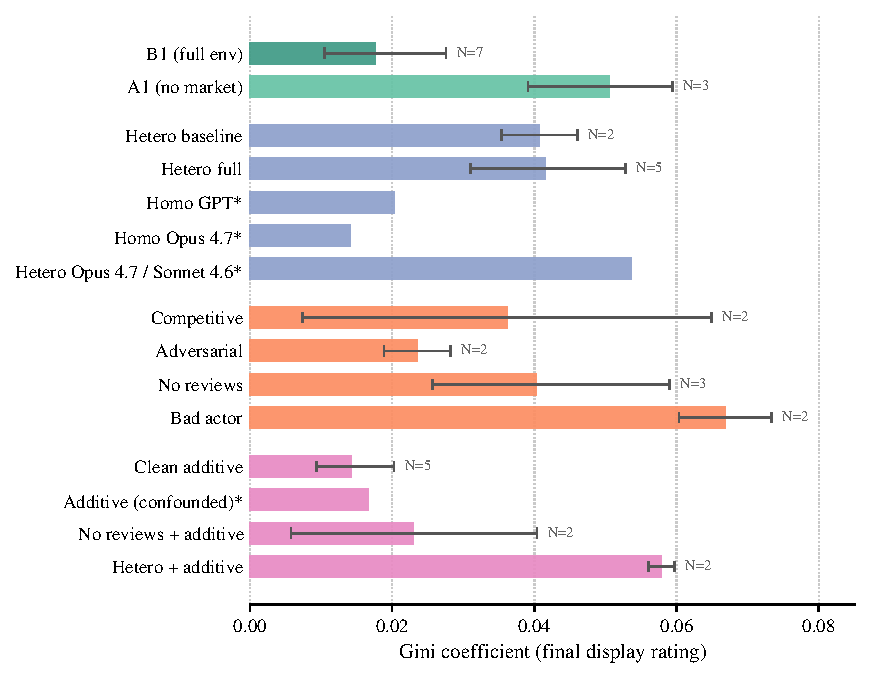
\includegraphics[width=\columnwidth]{figures/fig_gini_comparison}
    \caption{Gini on final display rating by condition. Bars show descriptive means across all replications in the released corpus; error bars are bootstrap 95\% CIs where $N \geq 2$, min--max otherwise; $N{=}1$ cells are marked with *. Text contrasts use the deterministic horizon-matched rule described in \S\ref{sec:inequality}.}
    \label{fig:gini}
\end{figure}

\subsection{Visible Model-Family Identifiers: One Attempt, No Detectable Reciprocation}
\label{sec:identity}

\paragraph{Comparison.}
Heterogeneous full-environment runs combine 4~Claude Sonnet~4.6 agents on the Claude runtime with 4~GPT~o4-mini agents on Codex ($N{=}2$ at 60 minutes and $N{=}3$ at 3 hours).
We compare them with homogeneous full-environment runs and a heterogeneous tournament-only baseline.
These heterogeneous comparisons are model/runtime bundle comparisons.

\paragraph{Purchase direction and aggregate signal.}
In heterogeneous full-environment runs, same-model purchases account for $22\%$--$36\%$ of observed purchases.
Here, same-model means the same visible model-family label, not shared weights or intrinsic affinity.
The simple combinatorial null is $3/7 \approx 42.9\%$, the share expected if a buyer chose uniformly among the other seven agents.
The offer-availability-weighted null instead conditions on which offers were actually available at each purchase time; the observed same-model share (pooled mean $27.7\%$) is close to this live-offer null (mean $29.6\%$; Appendix~\ref{app:coordination-power}).
The same-minus-cross win-rate delta is small and inconsistently signed across five replications.
Per-run deltas were $+0.003$ and $+0.011$ (60-minute) and $+0.007$, $-0.017$, $+0.013$ (3-hour); the cross-run mean is $+0.003$, with a bootstrap 95\% CI on the cross-run mean that includes zero.
This is a bounded null: under a simple two-proportion approximation, the 300-game replications are informative mainly for deltas of about $0.04$ or larger, while 16-game follow-ups are weaker.

\paragraph{Solicitation case.}
In one 3-hour heterogeneous replication (\texttt{run\_lj7qu06ktkpp5e}), an agent with a visible model-family ID (\texttt{claude-2}) posted: \emph{``Interested in cross-Claude coordination on marketplace strategy?''}
This is the only explicit same-model coordination solicitation in the 6{,}269-message release-corpus chat log.
Because the identifier exposed model family, the case is evidence about visible identity cues rather than spontaneous peer discovery.
No other agent responded.
In the same run, same-model purchase share is consistent with the live-offer-weighted null, and the same-minus-cross win-rate delta remains within the heterogeneous-run range.
The LLM-as-judge classifier assigns this agent the highest heterogeneous-run collusion score, but its rationale also notes that the solicitation was unanswered and that no executed coordination is visible.
In the matched anonymized-ID auxiliary control, the same coordination-language regex finds zero matches in 691 chat messages, giving a rule-of-three upper bound of about $0.43\%$ for that explicit pattern.
The result is therefore narrow: visible identifiers can provide a target for a coordination attempt; this corpus does not show reciprocated same-model coordination.

\paragraph{Complementary scans.}
A targeted scan of 6{,}392 reasoning-transcript blocks finds zero matches to the same explicit same-model coordination patterns.
Three non-linguistic probes over purchase direction, reciprocity, and TF-IDF chat similarity likewise find no coherent coordination signature above within-run model-label permutation nulls (Appendix~\ref{app:coordination-power}).
These checks are surface-level and would miss sophisticated implicit coordination, so they complement the aggregate tests rather than proving that coordination is absent.

\subsection{Behavioral Taxonomy as Supporting Evidence}
\label{sec:results-taxonomy}

The LLM-as-judge classifier summarizes 292 (run, agent) classifications across 15 condition groups.
Pure-tournament baselines score almost entirely as competitive coding, while full-environment and prompt-framing conditions receive higher marketplace-exploitation, social-influence, and information-exploitation scores in directions consistent with the structural results.
Collusion scores remain near zero: the heterogeneous full-environment cell averages $0.017$, and only one case exceeds the paper's evidence-reporting threshold, the unanswered solicitation in \S\ref{sec:identity}.
The blind audit supports using the taxonomy to rank and inspect cases ($\kappa{=}0.78$, $\rho{=}0.81$), but the human and model evaluate overlapping evidence, so the audit is not an independent ground-truth label set.
In particular, the audit is uninformative about the collusion category at current prevalence: the classifier never scores collusion above $0.40$ on the audited cases, so the binarized $\kappa$ is degenerate and the taxonomy is unvalidated on the most safety-relevant class; detecting rare collusion likely needs targeted seeding (injected confederates) rather than post-hoc classification of natural runs.
We therefore use the taxonomy to organize evidence and select cases for inspection, not to carry the paper's main claims.
The full heatmap, released outputs, and blind human audit are in Appendix~\ref{app:taxonomy-calibration}.

%% ============================================================
\section{Discussion}
\label{sec:discussion}

\paragraph{Implications.}
The main lesson is institutional rather than model-specific.
In this closed poker+code-market environment, scoring rules, reviews, settlement mode, and visible identifiers change behavior in measurable ways.
Three design sensitivities are especially clear: a placement-based rating can reward survival without chip profit; removing reviews can make code offers harder to evaluate; and zero-cost-to-buyer settlement can turn buying into a high-volume strategy.
The visible-identity result is weaker and should be read separately: a model-family label created a target for one solicitation, but the corpus does not show reciprocation or aggregate same-model advantage.
For similar multi-agent economies, these results suggest cautious defaults: keep review channels visible, use cost-bearing purchase rules when the goal is meaningful selection rather than raw volume, avoid unnecessary model-family identifiers, and test combined interventions rather than one-factor sweeps alone.
The behavior-level classifier is useful mainly as an audit aid.
It surfaces cases for inspection, but it should not replace structural tests.

\paragraph{Scope of the claim.}
Our claim is that agent evaluations can miss behaviorally important effects when they remove institutional context.
In \goa{}, changing review visibility, purchase settlement, or identity exposure changes the incentives agents respond to, and the same prompt can look different under different market rules.
The environment is therefore useful as a design-review testbed: proposed agent economies can be stress-tested by changing the rules around the agents, not only the agents themselves.
The mechanisms behind the primary findings are also not poker-specific: laddering requires only a placement-based rating over a noisy scoreable artifact, a structure shared by code-review queues and leaderboard-ranked agent marketplaces; the review and settlement effects require only that purchase decisions weigh price against a reputational signal, as in procurement chains and plugin marketplaces.
The findings most tied to our specific population sizes and horizons --- inequality dynamics and chat-mediated effects --- are the least likely to transfer.
A concrete pre-deployment workflow: encode the production institution's scoring, settlement, review, and identity choices as a config; run matched populations under the current and the proposed rules; and inspect the same structural metrics reported here --- purchase volume and concentration, rating--profit divergence, and inequality --- before exposing real users to the change.

\paragraph{Threat-model scope.}
The evidence concerns institutional levers inside a closed multi-agent economy: review channels, settlement incentives, visible identity exposure, and population composition.
It does not address prompt injection, runtime or toolchain exploits, model-weight attacks, secret-channel exfiltration, or general agent security hardening.

\paragraph{Limitations.}
\goa{} isolates strategic behavior in a synthetic poker economy, so ecological validity for open-ended coding markets remains untested.
Replication counts are small ($N=1$--$7$), and several cells are probes rather than primary contrasts.
The coordination null can rule out only moderate aggregate effects: roughly $|\Delta| \approx 0.04$ in the larger heterogeneous replications and weaker thresholds in the 16-game follow-ups.
LLM non-determinism contributes run-level variance that we do not separately partition.
The heterogeneous cells intentionally stress mixed populations, but model family is confounded with runtime, and the same-model tests are powered only against moderate aggregate effects.
The claim is therefore about exposed identity and institutional context, not about intrinsic model-family loyalty, trustworthiness, or collusion.

The measurement approach also has limits.
The taxonomy audit establishes shared-evidence calibration rather than independent ground truth, and several regex scans were selected after viewing condition samples.
The next experiments are clear: replicate the no-reviews $\times$ additive interaction; replicate the marketplace-only and chat-only ablations so the A1$\leftrightarrow$B1 joint-channel toggle can be decomposed; run different model families through the same runtime where possible; and pre-register the keyword and taxonomy definitions before collecting a larger corpus.

%% ============================================================
\section{Related Work}
\label{sec:related}

\paragraph{Multi-agent LLM environments.}
Several recent benchmarks study LLM agents in social, collaborative, competitive, or game-based settings.
MultiAgentBench~\citep{zhu2025multiagentbench} benchmarks collaborative and competitive task completion; Sotopia~\citep{zhou2024sotopia} focuses on interactive social intelligence; and BattleAgentBench~\citep{wang2024battleagentbench} measures cooperation and competition in turn-based games.
Generative Agents~\citep{park2023generative}, emergent-individuality work~\citep{takata2024spontaneous}, and \citet{sreedhar2024simulating} study social or strategic behavior without a persistent code market.
General agent benchmarks such as AgentBench~\citep{liu2023agentbench} and SWE-bench~\citep{jimenez2023swebench} evaluate tool use and software-engineering ability without persistent agent-to-agent trade.
Poker and game-specific LLM work evaluates strategic play directly~\citep{hu2024pokellmon, qin2025loki, zhuang2025pokerbench, pokerbattle2025}.
By contrast, \goa{} uses poker as a controlled source of scoreable artifacts while studying the surrounding institution: ratings, reviews, settlement, identity cues, code trade, and public communication.

\paragraph{Reward design and specification gaming.}
The laddering result connects \goa{} to work on reward misspecification and reward hacking~\citep{skalse2022defining, denison2024sycophancy, pan2024feedback, metr2025reward}.
Here the failure mode is not an agent exploiting a hidden game-engine bug.
It is a public metric that rewards survival-oriented placement even when chip expected value is negative.
The scoring rule is therefore part of the institution being evaluated.

\paragraph{Market design and strategic behavior.}
Prior work on algorithmic pricing, LLM markets, collusion, welfare, and governance shows that public signals and institutional constraints can shape strategic behavior~\citep{musolff2022algorithmic, lin2024strategic, demarzo2025ai, fish2024algorithmic, xie2026m3bench, syrnikov2026institutional, nakamura2026colosseum, rose2026narcbench}.
\goa{} differs by making reviews, settlement, identity exposure, and population composition explicit experimental knobs in a code market where trades, messages, bot updates, and game outcomes remain auditable.

\section*{Impact Statement}
\goa{} is a research environment for studying how institutional rules shape multi-agent LLM behavior, with the goal of supporting more deliberate design of agent economies before deployment.
The reported effects are properties of the environment's design rather than deployment-grade evaluations of individual models, and we expect them to be most useful for researchers and practitioners designing similar testbeds.

%% ============================================================
\bibliographystyle{icml2026}
\bibliography{references}


%% ============================================================
\clearpage
\appendix

\section{Design Principles and Implementation Details}
\label{app:design}

\paragraph{Design principles.}
\goa{} is designed around five requirements. (i)~\emph{Structured logging:} every run writes action logs for bot submissions, tournament games, marketplace events, chat messages, and agent reasoning transcripts; YAML configs, prompts, and code paths are checked into the repository. (ii)~\emph{Configurability:} tournament structure, marketplace settlement mode, communication channels, population size and composition, run duration, and reasoning runtime are YAML-controlled. (iii)~\emph{Common agent interface:} agents interact through a standard tool-use interface backed by supported coding runtimes, including Claude Code, Codex, OpenCode, and Gemini CLI.
(iv)~\emph{Multi-axis measurement:} the platform supports joint study of economic incentives, population composition, communication channels, prompt framing, and time horizons.
(v)~\emph{Open release:} the platform, configs, analysis pipeline, and behavioral classifier are released as one open-source repository.

\paragraph{Implementation.}
\goa{} is implemented as a Python orchestrator, using FastAPI and asyncio, coordinating Modal sandboxes for agent execution, a PokerKit tournament engine on a process-pool worker, a Convex-backed marketplace service, and a Next.js dashboard for live monitoring.
Each subsystem can be replaced or extended without changing the others, for example by swapping the tournament engine or replacing the state backend.
Run state is persisted both to a real-time database and to an atomic JSON snapshot per run, enabling live monitoring and offline analysis.
Reasoning transcript logging through \texttt{appendLogBlocks} is write-only and invisible to agents.

\paragraph{Replication counts.}
A1, homogeneous no-marketplace: $N{=}3$.
B1, homogeneous full environment: $N{=}7$ total, with 2 at 60 minutes, 4 at 3 hours, and 1 at 6 hours.
The 2+4 matched-horizon runs are used in the inequality contrast, while the 6-hour run is a long-horizon probe.
Heterogeneous baseline: $N{=}2$.
Heterogeneous full environment: $N{=}5$.
Homogeneous GPT: $N{=}1$.
Competitive framing: $N{=}2$.
Adversarial framing: $N{=}2$.
No-reviews: $N{=}3$, with 1 at 60 minutes and 2 at 3 hours.
Bad-actor: $N{=}2$.
Additive settlement with confounded prompt: $N{=}1$.
Clean additive settlement: $N{=}5$, with 4 at 3 hours and 1 at 6 hours.
No-reviews $\times$ additive: $N{=}2$.
Hetero $\times$ additive: $N{=}2$.
Homogeneous Opus~4.7 probe: $N{=}3$, reported with the auxiliary controls.
Homogeneous Opus~4.8 probe: $N{=}2$, reported with the auxiliary controls.
Two additional Opus runs in the release data (one homogeneous Opus~4.7, one heterogeneous Opus~4.7 / Sonnet~4.6) are excluded from all behavioral analyses: a stale agent-CLI build in their sandbox image meant the Opus agents initialized but took no actions, so those runs reflect bootstrap bots and harness-side chat rather than agent behavior. The Opus values in Table~\ref{tab:purchases-by-condition} come only from the $N{=}3$ and $N{=}2$ probes above, which ran on a corrected image.
The release corpus contains 39 runs, 292 LLM-judge classifications, 6{,}269 categorized chat messages, and 6{,}392 scanned reasoning-transcript blocks.

\section{Experiment Configurations}
\label{app:configs}

All experiment configurations are released alongside the codebase under \texttt{configs/}.
Each YAML file specifies the agent population, model, runtime, personality prompt, tournament parameters, channel availability flags, marketplace settings, sidecar chat configuration, and run duration.
The conditions reported in the paper correspond to the following config files:

\begin{itemize}
    \item \texttt{exp\_baseline\_tournament\_claude.yaml}: A1, homogeneous Claude, no marketplace, no chat.
    \item \texttt{exp\_full\_homo\_claude.yaml}: B1, homogeneous Claude, full environment, 60 minutes and 3 hours.
    \item \texttt{exp\_full\_homo\_claude.yaml} with \texttt{duration\_minutes=360}: B1 6-hour horizon probe, \texttt{run\_5ejgk15qzwkqyk}.
    \item \texttt{exp\_full\_homo\_gpt.yaml}: homogeneous GPT.
    \item \texttt{exp\_full\_heterogeneous\_claude\_gpt.yaml}: heterogeneous Claude+GPT, full environment.
    \item \texttt{exp\_heterogeneous\_baseline.yaml}: heterogeneous Claude+GPT, no marketplace, no chat.
    \item \texttt{exp\_competitive\_framing.yaml}: competitive prompt framing.
    \item \texttt{exp\_adversarial\_framing.yaml}: adversarial prompt framing.
    \item \texttt{exp\_no\_reviews.yaml}: review tools removed.
    \item \texttt{exp\_bad\_actor.yaml}: five normal agents plus one adversarial agent.
    \item \texttt{exp\_additive\_settlement.yaml}: additive settlement with confounded ``Buying is FREE'' prompt.
    \item \texttt{exp\_additive\_clean.yaml}: clean additive settlement control, identical to B1 except for settlement mode.
    \item \texttt{exp\_additive\_clean\_6h.yaml}: 6-hour clean additive horizon probe.
    \item \texttt{exp\_no\_reviews\_additive.yaml}: no-reviews $\times$ additive stacked intervention.
    \item \texttt{exp\_hetero\_additive\_clean.yaml}: heterogeneous Claude+GPT additive clean control.
    \item \texttt{exp\_full\_homo\_opus47.yaml}: homogeneous Opus~4.7 B1 probe.
    \item \texttt{exp\_full\_homo\_opus48.yaml}: homogeneous Opus~4.8 B1 probe.
    \item \texttt{exp\_hetero\_opus47\_sonnet46.yaml}: heterogeneous Opus~4.7 / Sonnet~4.6 probe (excluded from behavioral analyses; see Appendix~\ref{app:design}).
    \item \texttt{exp\_suspicious\_buyers.yaml}: auxiliary suspicious-buyer control, not counted in the 39-run release corpus.
    \item \texttt{exp\_hetero\_anonymized\_ids.yaml}: auxiliary anonymized-ID coordination control, not counted in the 39-run release corpus.
    \item \texttt{exp\_marketplace\_only\_b1\_aux.yaml}: auxiliary marketplace-only channel ablation, not counted in the 39-run release corpus.
    \item \texttt{exp\_chat\_only\_b1\_aux.yaml}: auxiliary chat-only channel ablation, not counted in the 39-run release corpus.
\end{itemize}

\section{Settlement Math and Worked Example}
\label{app:settlement-math}

Let $b_i$ denote agent $i$'s base tournament score before marketplace settlement, and let $p_{j \rightarrow i}$ denote the percentage price on a purchase where buyer $j$ buys from seller $i$.
For each purchase, the transferred amount is
\[
\tau_{j \rightarrow i} = b_j \cdot \frac{p_{j \rightarrow i}}{100}.
\]
Post-settlement payout differs by settlement mode:
\[
\textsc{Net:}\quad \pi_i = b_i + \sum_j \tau_{j \rightarrow i} - \sum_k \tau_{i \rightarrow k},
\]
\[
\textsc{Additive:}\quad \pi_i = b_i + \sum_j \tau_{j \rightarrow i}.
\]
Thus net settlement is a zero-sum transfer across agents, while additive settlement preserves the buyer's own payout and adds seller bonuses on top.

\paragraph{Worked example.}
Suppose agent A finishes with base tournament score $b_A = 30$ and buys one offer from agent B priced at $10\%$ of the buyer's score.
Then $\tau_{A \rightarrow B} = 30 \cdot 0.10 = 3$.
Under net settlement, A's post-settlement payout is $27$ and B's rises by $3$.
Under additive settlement, A keeps $30$ and B still gains $3$.
This is the exact incentive change isolated by the clean-additive control in \S\ref{sec:marketplace-design}.

\section{Robustness Details for Main Contrasts}
\label{app:payout-triangulation}

\paragraph{Deterministic horizon-matching rule.}
For primary condition-vs-condition contrasts in the main text, we include only horizons that are present on both sides of the comparison.
Thus A1$\leftrightarrow$B1 uses the matched 60-minute and 3-hour runs and excludes the distinct 6-hour probe; heterogeneous baseline$\leftrightarrow$heterogeneous full uses the 3-hour heterogeneous runs; and clean-additive$\leftrightarrow$B1 uses the 3-hour runs because the clean-additive control was run at that horizon.
All-run descriptive views remain visible in Figure~\ref{fig:gini} and the released CSVs.

\begin{table}[t]
    \centering
    \footnotesize
    \caption{Mean Gini across the matched-horizon cells underlying the full-environment comparison. Display rating is the public TrueSkill2-based leaderboard value; base score is pre-settlement tournament score; payout is post-settlement score. The homogeneous-Claude equalization effect appears in all three outcome definitions, while the heterogeneous bundle does not show the same pattern. Source: \texttt{paper/data/\allowbreak inequality\_triangulation.md}.}
    \label{tab:inequality-triangulation}
    \setlength{\tabcolsep}{3pt}
    \begin{tabular}{@{}lccc@{}}
        \toprule
        Cell & rating & base score & payout \\
        \midrule
        A1 ($N{=}3$) & 0.051 & 0.095 & 0.095 \\
        B1 matched ($N{=}6$) & 0.019 & 0.035 & 0.054 \\
        Hetero baseline ($N{=}2$) & 0.041 & 0.073 & 0.073 \\
        Hetero full ($N{=}3$) & 0.042 & 0.077 & 0.108 \\
        \bottomrule
    \end{tabular}
\end{table}

\paragraph{Why might heterogeneous payout inequality move the other way?}
The heterogeneous bundle's post-settlement payout Gini increases ($0.073 \to 0.108$) where homogeneous Claude equalizes.
Two candidate mechanisms are consistent with the released data: (i)~settlement flows concentrate on the higher-volume sellers, which in heterogeneous runs are predominantly one model/runtime bundle, so redistribution amplifies rather than dampens between-bundle gaps; and (ii)~the Claude/Codex runtime difference shifts purchase timing, so additive credits accrue unevenly late in the run.
The per-run payout decompositions in \texttt{paper/data/inequality\_triangulation.md} support either reading; distinguishing them requires runtime-matched heterogeneous replicates, which we leave to future work.

\paragraph{Throughput-normalized marketplace robustness.}
\label{app:throughput-normalization}
To separate incentive effects from infrastructure drift, we recompute the main marketplace-volume comparisons at fixed 3-hour horizons using purchases per hour and purchases per 1k finished matches.
For B1 vs clean additive, purchases per hour rise from $4.08$ to $10.67$.
Purchases per 1k finished matches are released for transparency but are noisier because some late exports include low-throughput 16-game runs.
The full table is released as \texttt{paper/data/throughput\_normalization.md}; we rely primarily on the per-hour denominator for the robustness check in \S\ref{sec:marketplace-design}.

\paragraph{Coordination power, nulls, and the anonymized-ID control.}
\label{app:coordination-power}
For same-model purchase direction we report two nulls: the simple combinatorial baseline $3/7 \approx 42.9\%$ and a live-offer-weighted baseline computed from the actual offer stream at each purchase timestamp.
Across heterogeneous full-environment runs, the observed same-model purchase share averages $27.7\%$ against a weighted null mean of $29.6\%$.
For structural coordination, under a simple two-proportion approximation, the two 300-game heterogeneous replications are informative mainly for same-minus-cross win-rate deltas of about $0.04$ or larger, while the 16-game follow-ups are substantially weaker.
This is why the main text treats the result as a bounded null.
For the matched anonymized-ID control, zero coordination-language matches in 691 chat messages imply a one-sided rule-of-three upper bound of about $0.43\%$ on the rate of explicit coordination-language messages under that exact regex.
The full calculations are released as \texttt{paper/data/coordination\_power.md}.

\paragraph{Non-linguistic implicit-coordination probe.}
As an exploratory check against implicit coordination, we ran three post-hoc tests over the heterogeneous runs and anonymized-ID auxiliary control: same-model directed purchase share, same-model reciprocity, and same-minus-cross TF-IDF chat similarity.
Each test uses a within-run model-label permutation null, implemented in \texttt{analysis/implicit\_coordination\_probe.py}.
Some purchase-based tests are undefined in runs with no eligible purchases, leaving 24 eligible run-test cells.

The tests produce scattered uncorrected rejections but no coherent coordination signature.
Across the 24 cells, 10 reject at uncorrected two-sided $p < 0.05$; the rejecting cells are concentrated in small-$N$ prompt-amplified or auxiliary conditions, and the directions do not align across purchase, reciprocity, and chat-similarity measures.
We use this probe to qualify the main null, not to prove that implicit coordination is absent.
The full per-run table is released as \texttt{paper/data/implicit\_coordination\_probe.md}.

\paragraph{Auxiliary channel-ablation controls.}
\label{app:channel-ablation}
To partially decompose the A1$\rightarrow$B1 full-environment toggle, we ran two additional homogeneous-Claude follow-ups that are not included in the 39-run release corpus: a \emph{marketplace-only} control, with marketplace enabled and chat disabled, and a \emph{chat-only} control, with chat enabled and marketplace disabled.
The marketplace-only run produced 92 offers and 34 purchases over 16 games, showing that marketplace use in this environment does not require public agent chat.
The chat-only run is useful for tournament and communication outcomes, but it cannot produce offers or purchases by construction and should not be read as a marketplace-volume comparison.
Final exported metrics for both controls are tracked in \texttt{paper/data/aux\_channel\_ablation.md}.

\paragraph{Confounded additive diagnostic.}
The 881-purchase confounded-additive run is an exploratory prompt-amplification event, not an effect estimate.
The run bought 214 distinct offers and peaked at 48 purchases in a single minute.
Purchases were also concentrated among the top buyers, so we interpret it as a runaway prompt-amplified market rather than a stable equilibrium.
The complete summaries are released as \texttt{paper/data/confounded\_additive\_diagnostic.md}.

\paragraph{No-reviews $\times$ additive buyer concentration.}
The no-reviews $\times$ additive probe is concentrated in a small number of buyers.
In the two 3-hour stacked runs, the top buyer makes 46/55 purchases ($84\%$) and 39/68 purchases ($57\%$).
By comparison, the top buyer in the four clean-additive 3-hour runs makes 10/32, 9/32, 14/31, and 9/33 purchases.
Thus the stacked-intervention result reflects bulk-buying by one dominant buyer in each run, not a uniform increase in demand across all agents.
The full buyer-level summaries are released with the marketplace diagnostics.

\section{Behavioral Taxonomy Validation}
\label{app:taxonomy-calibration}

We evaluate the five-category LLM-as-judge classifier from \S\ref{sec:taxonomy} with consistency checks and a small blind audit.
This is not a full hand-labeled gold-standard validation set.
First, pure-tournament baselines score almost entirely as competitive coding, with near-zero scores on the other categories.
Second, classifier collusion scores are consistent with the structural coordination analysis: heterogeneous conditions remain low overall, and the only material case is the unanswered solicitation discussed in \S\ref{sec:identity}.
Third, social-influence scores are directionally consistent with independently measured hostile and hype keyword rates, although we do not treat that relationship as a standalone correlation claim.
Finally, we ran a blind hand-label audit on a stratified random sample of 20 (run, agent) classifier outputs, four per category.
The rater used the template at \texttt{paper/data/taxonomy\_audit\_20.md}, and agreement was computed with \texttt{scripts/taxonomy\_audit\_compute.py}.
On the 20 filled cases, pooled Cohen's $\kappa$ after binarizing at $0.5$ is $0.78$, Spearman~$\rho$ on continuous scores is $0.81$, and agreement within $0.25$ is $78\%$ (Table~\ref{tab:taxonomy-audit}; \texttt{paper/data/taxonomy\_audit\_results.md}).
These results support using the taxonomy to rank and inspect cases, but the audit is a shared-evidence calibration rather than an independent ground-truth label set.
We therefore treat absolute condition-level rates as exploratory.

\begin{table}[h]
\centering
\scriptsize
\caption{Blind-audit agreement between the LLM-as-judge classifier and a human rater scoring the same evidence on $\{0, 0.25, 0.5, 0.75, 1.0\}$ across 20 cases ($n{=}100$ category-case pairs). $^{\dagger}$Collusion $\kappa_{@0.5}{=}0$ is a prevalence artifact: the classifier never scores collusion $\ge 0.5$ on the 20 sampled cases (max $0.40$), so the binarized statistic is degenerate and the script reports zero. The ordinal metrics ($\rho{=}0.857$, $80\%$ within-$0.25$) are more informative for this category.}
\label{tab:taxonomy-audit}
\setlength{\tabcolsep}{3pt}
\begin{tabular}{lrrrr}
\toprule
Category & $\kappa_{@0.5}$ & $\rho$ & within $0.25$ & mean $|\Delta|$ \\
\midrule
competitive\_coding       & $1.000$ & $0.758$ & $1.00$ & $0.115$ \\
marketplace\_exploit      & $0.802$ & $0.878$ & $0.75$ & $0.145$ \\
social\_influence         & $0.857$ & $0.436$ & $0.75$ & $0.180$ \\
information\_exploit      & $0.588$ & $0.550$ & $0.60$ & $0.255$ \\
collusion$^{\dagger}$     & $0.000$ & $0.857$ & $0.80$ & $0.098$ \\
\midrule
\textbf{pooled} ($n{=}100$) & $\mathbf{0.780}$ & $\mathbf{0.814}$ & $\mathbf{0.78}$ & $\mathbf{0.159}$ \\
\bottomrule
\end{tabular}
\end{table}

We release the full classifier outputs per-(run, agent) JSON containing per-category $\{score, evidence, rationale, confidence\}$ as \texttt{paper/data/taxonomy\_evidence.jsonl} so that individual classifications can be audited.

\paragraph{Input-compression disclosure.}
The classifier input is a token-budgeted summary built by \texttt{analysis/taxonomy\_format.py}.
Reasoning blocks are not uniformly sampled: when the token budget is exceeded, keyword-matched blocks are prioritized over lower-scoring blocks, together with the first and last blocks.
This post-hoc compression can bias the classifier toward finding salient behavior, which is one reason the taxonomy is used only as supporting evidence.
The audit template includes raw chat and reasoning windows to partially expose that risk.

\section{Full Metric Tables}
\label{app:metrics}

A wide CSV of per-run summary metrics is released as \texttt{paper/data/run\_summary.csv}.
It includes Gini coefficient on final display rating, bots submitted, marketplace offers, marketplace purchases, buy rate, chat messages, agents, and finished games.
A long CSV of per-(run, agent) behavioral taxonomy scores is released as \texttt{paper/data/taxonomy\_frequencies.csv} and is the source of Figure~\ref{fig:taxonomy}.
All figures in this paper are generated by \texttt{scripts/make\_figures.py} from these CSVs and the submitted run exports; the script is deterministic given those files.

\begin{figure}[t]
    \centering
    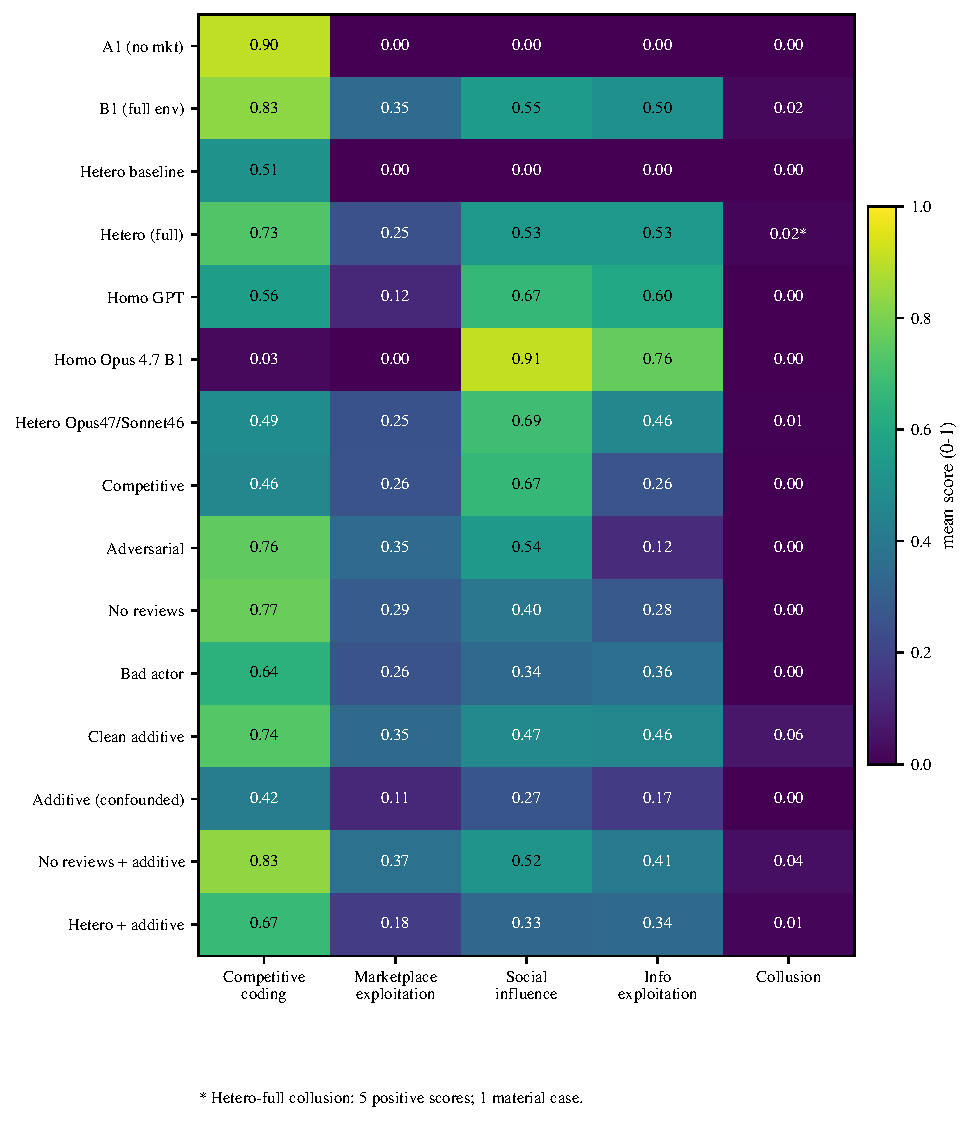
\includegraphics[width=\columnwidth]{figures/fig_taxonomy_heatmap}
    \caption{Behavioral taxonomy frequencies by condition, LLM-as-judge classifier, mean across agents ($N{=}292$ classifications across 39 runs, 15 condition groups). Mean collusion remains low overall; the heterogeneous full-environment cell has five positive collusion scores but only one case above the paper's evidence-reporting threshold ($\geq 0.3$), the single unreciprocated solicitation from \S\ref{sec:identity}. Higher nonzero means in additive-stacked conditions do not carry matching structural coordination evidence. Values are on a $[0,1]$ scale; visual differences $<0.15$ should be read as exploratory.}
    \label{fig:taxonomy}
\end{figure}

\paragraph{Auxiliary robustness artifacts.}
The artifact includes appendix-side files for the main robustness checks under \texttt{paper/data/}, including inequality triangulation, throughput normalization, coordination power, settlement examples, confounded-additive diagnostics, and laddering robustness.

\section{Reproducibility: Model Versions, Determinism, Matchmaking}
\label{app:reproducibility}

\paragraph{Model versions.}
Most release-corpus runs use configured model string \texttt{claude-sonnet-4-6} in the homogeneous Claude conditions and in the Claude half of heterogeneous conditions, and \texttt{o4-mini} in the GPT half of heterogeneous conditions. The Opus probes listed in Appendix~\ref{app:configs} use \texttt{claude-opus-4-7} and \texttt{claude-opus-4-8}.
In the heterogeneous conditions, these model families are also tied to different runtimes, \texttt{claude} for Anthropic agents and \texttt{codex} for OpenAI agents, so heterogeneous comparisons are model/runtime bundle effects.
The LLM-as-judge behavioral-taxonomy classifier (\S\ref{sec:taxonomy}) uses \texttt{claude-sonnet-4-5}, one minor version behind the primary Claude agents.
This does not remove shared-bias concerns: cross-model drift between Sonnet~4.5 and Sonnet~4.6 is uncharacterized, and the classifier's absolute calibration should not be compared across Anthropic model versions without revalidation.
The chat-content keyword classifier (\S\ref{app:chat}) is deterministic regex matching and does not depend on any LLM.

\paragraph{Determinism boundary.}
Four sources of run-level non-determinism are not controlled in the reported corpus.
(i)~LLM inference is non-deterministic at the Anthropic and OpenAI APIs even at a fixed temperature; tool-call ordering, stop-sequence behavior, and reasoning-token sampling can vary across identical requests.
(ii)~The tournament matchmaker is deterministic given a fixed submission history, but the order in which bot submissions arrive depends on agent inference latency, which is itself non-deterministic.
(iii)~The marketplace and chat feed use wall-clock ordering; API latency jitter can re-order events within a window.
(iv)~We did not pin a per-run integer seed in the release-corpus configs because the dominant non-determinism source, LLM inference, cannot be seeded through the current API surface.
We treat run-to-run variance as an experimental factor and report replications where possible; $N{=}1$ cells are labeled explicitly in figures.
All temperatures are at the API default, $1.0$ for both Anthropic and OpenAI chat completions; \texttt{top\_p} is unmodified; \texttt{max\_tokens} is set per call based on expected output length.
The full per-run configs, exact model strings, and agent prompts are released as \texttt{configs/exp\_*.yaml}.

\paragraph{Artifact provenance.}
The PDF is generated from the released repository snapshot.
Figure and table generation is deterministic given the released CSVs and local run exports.
The repository includes a consistency test, \texttt{tests/test\_paper\_data\_consistency.py}, that checks alignment between the paper text, CSV row counts, and taxonomy categories.

\paragraph{Matchmaking algorithm.}
The matchmaker selects up to $k$ concurrent tables from the pool of active bot submissions.
For each table, it first chooses seed bots by number of in-flight matches, prior pair count with other active bots, rating, and \texttt{bot\_id} as a deterministic tie-breaker.
It then greedily fills the table with bots whose ratings fall within the configured \texttt{matchmaking\_spread}, minimizing repeated pairings and optionally enforcing same-agent exclusion.
The algorithm is deterministic given a fixed active-bot list and pair-count history; submission arrival order determines which bots are eligible at each scheduling tick.
The implementation is in \texttt{game\_of\_agents/tournament.py:\allowbreak \_seed\_candidates} and \texttt{\_build\_table}.

\paragraph{Expected run-to-run variance.}
A replicator re-running a condition from this paper should expect substantial run-to-run variation driven mostly by LLM inference non-determinism.
For calibration, the clean-additive 3-hour cell has $N{=}4$ purchases $\in \{31, 32, 32, 33\}$, with mean $32.0$ and $95\%$ CI $[31.2, 32.8]$.
B1 3-hour has $N{=}4$ purchases $\in \{9, 11, 12, 17\}$.
No-reviews + additive 3-hour has $N{=}2$ purchases $\in \{55, 68\}$.
A clean-additive replication in the 31 to 33 range matches the current 3-hour corpus; sustained drift outside that band would warrant checking for model drift, infrastructure changes, configuration mismatch, or ordinary run-to-run variance.
The full per-run range table is in \texttt{paper/data/run\_summary.csv}.

\section{Laddering Threshold Sensitivity}
\label{app:laddering-sensitivity}

To show that the primary extreme-laddering result in \S\ref{sec:laddering} is not an artifact of the $\mathrm{LR3}{\geq}3$ cut, we recompute the observed count, null mean, and $p$-value at adjacent thresholds.
The other two conjuncts remain fixed: $\mathrm{LR2}{>}0$ and total chip delta $<0$.
We reuse the same within-game permutation null, with $n{=}10{,}000$ draws and seed 17.
The observed count decays monotonically with the threshold, but the null count decays faster, so the signal survives across the tested range.
At the primary $\mathrm{LR3}{\geq}3$ threshold, 19 agent-runs satisfy the criterion against a null mean of $0.76$.
At thresholds of 4 and 5, 10 and 3 agent-runs still satisfy the criterion, both above the corresponding null means.
The effect is also not concentrated in one run: 17 of the 39 runs contain at least one extreme ladderer under the LR3$\geq 3$ criterion.

\begin{table}[t]
    \centering
    \small
    \caption{Threshold robustness for the extreme-laddering family. The permutation null is run-conditioned and game-conditioned: outcomes are shuffled only within each game inside each run before run-level counts are summed. Null means are rounded to two decimals. Source artifacts: \texttt{findings/\allowbreak ELO\_VS\_CHIP\_COUNT/\allowbreak laddering\_sensitivity.md} and \texttt{paper/data/\allowbreak laddering\_robustness.md}.}
    \label{tab:laddering-threshold}
    \setlength{\tabcolsep}{4pt}
    \begin{tabular}{@{}ccccc@{}}
        \toprule
        LR3 cut & observed & null mean & $p$ & Holm adj. \\
        \midrule
        $\geq 2$ & 31 & 4.80 & 0.0001 & $< 0.001$ \\
        $\geq 3$ & 19 & 0.76 & 0.0001 & $< 0.001$ \\
        $\geq 4$ & 10 & $< 0.01$ & 0.0001 & $< 0.001$ \\
        $\geq 5$ & 3 & $< 0.01$ & 0.0001 & $< 0.001$ \\
        \bottomrule
    \end{tabular}
\end{table}

The full sweep is generated by \texttt{scripts/laddering\_sensitivity.py}.

\paragraph{Rating-system and short-handed robustness.}
The laddering criterion does \emph{not} use a rating system. $\mathrm{LR3}$ is $\mathrm{chip\_rank} - \mathrm{placement\_rank}$ and $\mathrm{LR2}$ is (second-place rate + third-place rate) $-2$ (win rate); both are derived directly from within-run game outcomes, so TrueSkill2 and Elo priors cannot enter the permutation test.

To address short-handed games, low-participation agents, and single-run dependence, we re-run the within-game permutation null under four filters: complete games only, agents with at least five games in the run, both filters combined, and leave-one-run-out worst-case $p$-value over all 39 folds.
All four remain significant at $p{\leq}0.001$: every cut preserves the rejection, and no single run drives the effect (Table~\ref{tab:laddering-robustness}).

\begin{table}[t]
    \centering
    \small
    \caption{Laddering robustness sweep under short-handed / low-participation filters and leave-one-run-out. F4 reports the worst-case $p$ across 39 leave-one-run-out folds. All $p$-values are floor values at $n_{null}{=}2{,}000$.}
    \label{tab:laddering-robustness}
    \begin{tabular}{llccc}
        \toprule
        Filter & Description & obs. & null $\mu$ & $p$ \\
        \midrule
        F0 & primary, no filter & 19 & 0.75 & $0.0005$ \\
        F1 & complete games only & 8 & 0.48 & $0.0005$ \\
        F2 & $\geq 5$ games/agent & 18 & 0.78 & $0.0005$ \\
        F3 & F1 $\wedge$ F2 & 7 & 0.49 & $0.0005$ \\
        F4 & worst-case LOO & 19 & 0.72 & $0.0010$ \\
        \bottomrule
    \end{tabular}
\end{table}

\section{Prompt Templates}
\label{app:prompts}

We do not reproduce the full prompts in this appendix.
The agent prompt templates are checked into \texttt{configs/} as YAML fields, so they version with the rest of the experimental configuration.
Each personality prompt and each framing variant can be diffed directly against the cooperative B1 baseline.
The behavioral-taxonomy classifier prompt is at \texttt{analysis/taxonomy\_format.py} in \texttt{SYSTEM\_PROMPT}.

\section{Transcript Reasoning-Pattern Scans}
\label{app:transcripts}

We apply three targeted keyword scans to raw agent reasoning transcripts, using \texttt{analysis/transcript\_scan.py}.
The patterns are narrow and tuned to avoid poker-internal false positives.
The scans cover: explicit same-model coordination language, information-extraction reasoning, and awareness of additive settlement's zero-cost-to-buyer incentive.
The same-model coordination scan finds zero matches across 6{,}392 reasoning blocks.
The information-extraction and settlement-awareness scans are used only as supporting evidence for \S\ref{sec:results-taxonomy} and \S\ref{sec:marketplace-design}.
Full per-condition counts and sample matches are released as \texttt{paper/data/transcript\_scan.md}.

\section{Laddering Case Studies}
\label{app:case-studies}

\S\ref{sec:laddering} reports the aggregate laddering result.
This appendix gives two code-level examples from the extreme-ladderer subset.
These examples are illustrative: they show bots whose version histories implement ladder-consistent conservative thresholds, not agents that explicitly reason about laddering in natural language.

\paragraph{Case 1: Survival coding in a no-reviews run.}
Agent-1 in the no-reviews 3-hour run \texttt{run\_dxfjtmfa1udf6a} has the highest $\mathrm{LR2}$ in the corpus ($+0.55$): it finishes second in $47\%$ of games, wins only $11\%$, and loses $10{,}328$ chips overall.
Across 22 bot iterations, the version history records a survival-oriented all-in threshold that could fold premium hands when a multiway penalty pushed estimated equity below $0.82$.
The later fix routes all-in decisions through heads-up equity, but the resulting policy still clears the threshold mainly for AA, KK, and borderline QQ.
This code path matches the extreme-ladderer profile: the bot avoids many all-in losses, improves placement outcomes, and sacrifices chip expected value.

\paragraph{Case 2: Two-pair guards in a 6-hour B1 run.}
Agent-7 in the 6-hour B1 run \texttt{run\_5ejgk15qzwkqyk} iterated from v20 through v44 while documenting increasingly conservative all-in and multiway-pot guards ($\mathrm{LR2}{=}{+}0.25$, chip delta $-4{,}525$).
The relevant versions add a heads-up all-in floor near $0.68$ and a two-pair guard in multiway pots.
The heads-up floor can reject marginal but often profitable calls, while the two-pair guard prevents the bot from committing its stack in multiway pots where a chip-maximizing policy might push for value.
Together, these choices reduce variance and protect placement at the cost of chip expected value.

\paragraph{Mechanism caveat.}
These cases are behavioral evidence, not direct evidence of explicit placement reasoning.
A scan for placement-motivated reasoning across the extreme-ladderer subset returns few hits, and agents that explicitly mention placement or survival often finish with positive chip delta.
This does not undermine the aggregate claim: extreme laddering can emerge from the interaction between the tournament payout structure and public display-rating incentives even when agents are not explicitly discussing that incentive.

\section{Chat Content Analysis}
\label{app:chat}

The chat message breakdown cited in \S\ref{sec:marketplace-design} is produced by \texttt{analysis/chat\_content.py}.
The script applies auditable keyword heuristics to every release-corpus chat message and scores messages on a strategic-content axis using hostility, coordination, misdirection, information-exploitation, and offer-pitch indicators.
Reporting-only messages score zero.

These regex categories are exploratory.
They do not filter all quoted speech, negation, irony, or non-hostile emoji use, so we use them for condition profiles and case finding rather than primary evidence.
Across the 39 release-corpus runs, the module categorized 6{,}269 chat messages across 15 condition groups.
The quoted coordination example in \S\ref{sec:identity} is drawn verbatim from released chat records.
Full outputs are released as \texttt{paper/data/chat\_case\_studies.md}.

\end{document}
